% -------------------------------------------------------------------
\chapter{Sensores de gases eletroquímicos}\label{apendix: sensores-ec}
% -------------------------------------------------------------------

Os sensores eletroquímicos funcionam baseados no princípio de conversão de energia química em energia elétrica e vice-versa, e consistem, basicamente, em uma célula contendo uma solução eletrolítica na qual são submersos eletrodos metálicos interconectados por um circuito externo \cite{Westbroek2005FundamentalsElectrochemistry}. Dentro da célula originam-se reações de oxidação–redução entre cada um dos eletrodos e a solução eletrolítica. As reações de redução removem elétrons do material do eletrodo, que passa a funcionar como catodo. Nas reações de oxidação, o eletrodo que faz o papel de anodo ganha elétrons e produz-se uma espécie oxidada. Esse intercâmbio de cargas entre os eletrodos e a solução analítica, equivalente a uma corrente elétrica fluindo do anodo para o catodo, é proporcional à velocidade das reações redox nas superfícies dos eletrodos \cite{R.Stetter2008AmperometricReview}. A Figura \ref{fig:celula-ec} mostra a estrutura básica de uma célula eletrolítica amperométrica de dois eletrodos.

\begin{figure}[htb]
	\caption{\label{fig:celula-ec}Representação de uma célula eletroquímica de dois eletrodos.}
	\begin{center}
		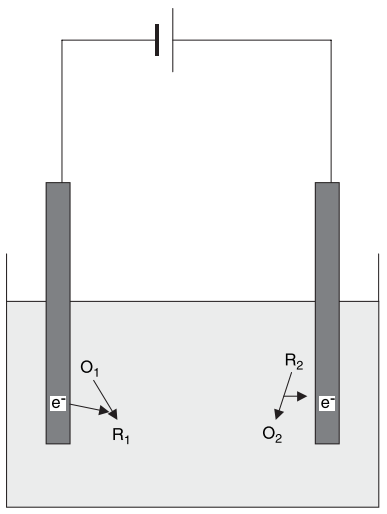
\includegraphics[width=0.6\textwidth]{aftertext/Operação sensores/Figuras/celula eletroquimica.PNG}
	\end{center}
	\fonte{\cite{Westbroek2005FundamentalsElectrochemistry}.}
\end{figure}

Segundo seu princípio de operação, os sensores eletrolíticos são classificados em amperométricos, potenciométricos e condutimétricos \cite{R.Stetter2008AmperometricReview}. Neste trabalho apenas são abordados os sensores amperométricos por serem os mais comumente utilizados no monitoramento de baixo custo.

Os sensores amperométricos apresentam uma estrutura básica de três eletrodos: o eletrodo de trabalho, o eletrodo contador e o eletrodo de referência. O eletrodo de trabalho é a superfície onde acontece a reação de interesse entre o material do eletrodo, a solução eletrolítica e o gás sob estudo, que formam uma interface de três fases. Para aumentar a seletividade dos sensores, costuma-se aplicar algum catalisador na superfície do eletrodo para facilitar ou catalisar determinadas reações. Como este eletrodo está em contato direto com o ar ambiente, corre risco de envenenamento se exposto a certos gases que possam ser adsorvidos no catalisador ou que possam reagir com ele produzindo outros compostos químicos que inibam sua ação \cite{Alphasense2013AlphasenseWork, Westbroek2005FundamentalsElectrochemistry, R.Stetter2008AmperometricReview,Baron2017AmperometricReview}.

A reação no eletrodo de trabalho pode ser de oxidação ou de redução, dependendo da natureza da substância gasosa de interesse. Na ausência de gás, a célula eletrolítica encontra-se em equilíbrio, mas, ao entrar em contato com a substância gasosa, as moléculas do gás produzem um desbalanço nas reações redox, e, como resultado, o eletrodo pode ganhar ou perder elétrons, obtendo assim uma carga elétrica \cite{Alphasense2013AlphasenseWork,R.Stetter2008AmperometricReview}.

A carga elétrica gerada no eletrodo de trabalho é balanceada com uma reação oposta no eletrodo contador. Se a reação no eletrodo de trabalho for de oxidação, então no contador se produzirá uma reação de redução complementar, e vice-versa. Como resultado, uma corrente elétrica é gerada, proporcional à velocidade das reações nas superfícies dos eletrodos, que por sua vez é proporcional à concentração do gás \cite{Alphasense2013AlphasenseWork,R.Stetter2008AmperometricReview,Westbroek2005FundamentalsElectrochemistry}.

Para assegurar que o sensor se encontra operando dentro de uma região de trabalho desejada, é utilizado o eletrodo de referência. Ele é encarregado de fixar a tensão do eletrodo de trabalho em um valor constante sem que este valor (i.e.: a tensão de operação) seja alterado pela circulação da corrente elétrica, entre os eletrodos contador e de trabalho, que resulta dos processos de transdução. Já o eletrodo contador é deixado com uma carga flutuante que dependerá unicamente das reações eletroquímicas decorrentes da exposição ao gás e do fluxo de elétrons resultante. A corrente de saída do sensor é o resultado da diferença de potencial entre os eletrodos contador e de trabalho \cite{Alphasense2013AlphasenseWork,Baron2017AmperometricReview}.

A corrente de saída dos sensores eletroquímicos é muito pequena, geralmente na ordem dos nanoamperes \cite{R.Stetter2008AmperometricReview}, fazendo necessária a utilização de uma etapa posterior de condicionamento. A função principal da etapa de condicionamento é transformar o valor da variável elétrica de saída do transdutor em um dado que possa ser lido por um sistema de aquisição e que represente a quantidade física sendo medida, em um determinado instante de tempo. Comumente, a saída da etapa de condicionamento é um sinal de tensão, ajustado para representar, proporcionalmente, dentro de um determinado intervalo, a variável física de interesse. Esse sinal de tensão pode então ser lido por um conversor analógico-digital. Adicionalmente, podem ser contempladas subetapas intermediária de amplificação, filtragem ou alisamento, ajuste de zero e de ganho, e linearização. 

No caso dos sensores eletroquímicos, a configuração mais utilizada no circuito de condicionamento é o potencióstato \cite{Alphasense2013AlphasenseWork,SPECSensors2016SPECConsiderations}. Este circuito controla o potencial aplicado aos eletrodos de trabalho e de referência e converte a corrente que circula entre os eletrodos de trabalho e contador em um valor de tensão proporcional. Um diagrama simplificado de um sensor eletroquímico e um potencióstato é ilustrado na Figura \ref{fig:condic-ec}.

\begin{figure}[htb]
	\caption{\label{fig:condic-ec}Potencióstato para condicionamento de sensores eletroquímicos.}
	\begin{center}
		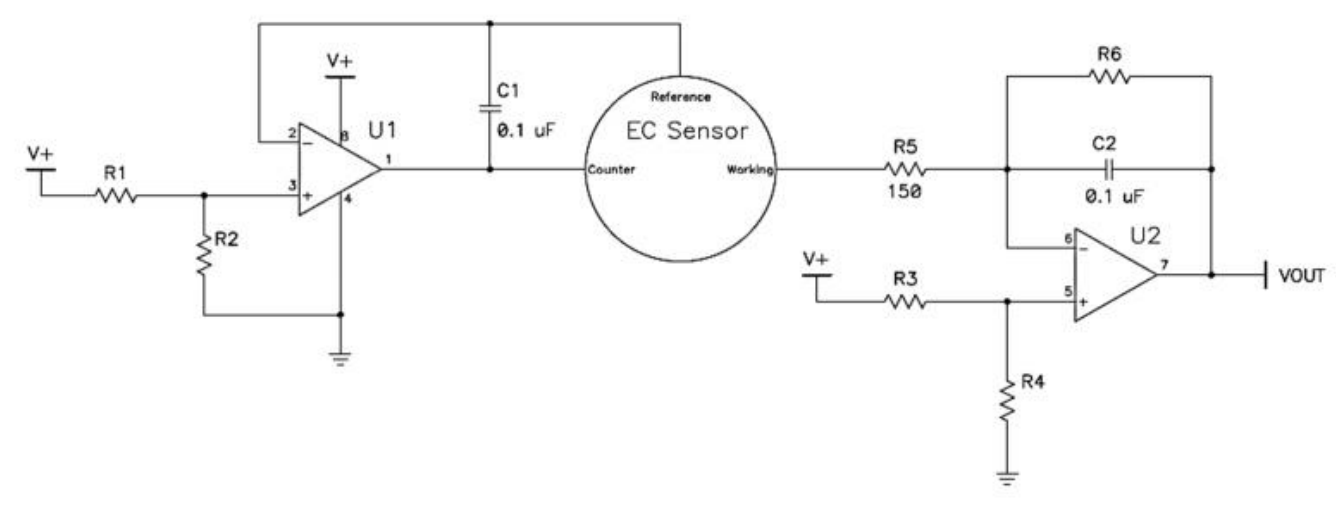
\includegraphics[width=\textwidth]{aftertext/Operação sensores/Figuras/Condicionamento SPEC.PNG}
	\end{center}
	\fonte{\cite{SPECSensors2016SPECConsiderations}.}
\end{figure}

O potencial do eletrodo de referência é estabelecido pelo amplificador U1 da Figura \ref{fig:condic-ec}, no pino 2. O amplificador U1 também garante a circulação da corrente elétrica pelo eletrodo contador, mantendo constante a tensão de referência. O amplificador U2 fixa o potencial do eletrodo de trabalho no pino 5, e converte em tensão (VOUT) a corrente que circula entre esse eletrodo e o contador. Dessa forma, é possível medir a tensão no pino VOUT como um valor proporcional à concentração do gás em contato com a superfície do sensor \cite{SPECSensors2016SPECConsiderations}.